% Typeset with XeTeX
% Allows use of system fonts rather than just LaTeX's ones
% NOTE - if you use TeXShop and Bibdesk (Mac), can complete citations
%  - open your .bib file, type~\citep{xx... and then F5 or Option-Escape
\documentclass[11pt]{article}
\usepackage[margin=1in, letterpaper]{geometry} % set page layout
%\geometry{letterpaper}  % or a4paper
\usepackage[xetex]{graphicx} % allows us to manipulate graphics.
% Replace option [] with pdftex if you don't use Xe(La)TeX
\usepackage{color}
\usepackage{indentfirst}
\usepackage{hyphenat}
\usepackage{epstopdf} % automatic conversion of eps to pdf 
\usepackage{amsmath, amssymb} % Better maths support & more symbols
\usepackage{textcomp} % provide lots of new symbols - see textcomp.pdf
% line spacing: \doublespacing, \onehalfspacing, \singlespacing
\usepackage{setspace}

\singlespacing
\usepackage{pgfplotstable}
% allows text flowing around figs
% use \begin{wrapfigure}{x}{width} where x = r(ight) or l(eft)
\usepackage{wrapfig}
\usepackage[parfill]{parskip} % don't indent new paragraphs
\usepackage{flafter}  % Don't place figs & tables before their definition 
\usepackage{verbatim} % allows \begin and \end{comment} regions
\usepackage{booktabs} % makes tables look good
\usepackage{bm}  % Define \bm{} to use bold math fonts
% linenumbers in L margin, start & end with \linenumbers \nolinenumbers,
\usepackage{lineno} % use option [modulo] for steps of 5
\usepackage[auth-sc]{authblk} % authors & institutions - see authblk.pdf
%\renewcommand\Authands{ and } % separates the last 2 authors in the list
% control how captions look; here, use small font and indent both margins by 20pt
\usepackage[small]{caption} 
\setlength{\captionmargin}{20pt}

%: FONT
% If you don't want to use system fonts, replace from here to 'Citation style' with \usepackage{Palatino} or similar
%: ************ FANCY FONTS START HERE
\usepackage[no-math]{fontspec} % 'no-math' = keep computer modern for math fonts
\usepackage{xunicode} % needed by XeTeX for handling all the system fonts nicely
\usepackage[no-sscript]{xltxtra} 
\setmonofont[Scale=0.8]{PT Serif} % typeface for \tt commands
\setsansfont[BoldFont={PT Serif Bold}, ItalicFont={PT Serif Italic}]{PT Serif} 
\defaultfontfeatures{Mapping=tex-text}
\setmainfont{Minion Pro}
%\setmainfont{Source Sans Pro}

%: ************ FANCY FONTS END HERE

%:CITATION STYLE
% natbib package: square,curly, angle(brackets)
% colon (default), comma (to separate multiple citations)
% authoryear (default),numbers (citations style)
% super (for superscripted numerical citations, as in Nature)
% sort (orders multiple cites into order of appearance in ref list, or year if authoryear)
% sort&compress: as sort, + multiple citations compressed (as 3-6, 15)
\usepackage[numbers,comma,sort&compress]{natbib}

%:SHORTCUT COMMANDS
% Maths
\newcommand{\ddt}[1]{\ensuremath{\frac{{\rm d}#1}{{\rm d}t}}}  % d/dt
\newcommand{\dd}[2]{\ensuremath{\frac{{\rm d}#1}{{\rm d}#2}}} % dy by dx  - \dd{y}{x}
\newcommand{\ddsq}[2]{\ensuremath{\frac{{\rm d}^2#1}{{\rm d}#2^2}}} % second deriv
\newcommand{\pp}[2]{\ensuremath{\frac{\partial #1}{\partial #2}}} % partial \pp{y}{x}
\newcommand{\ppsq}[2]{\ensuremath{\frac{\partial^2 #1}{\partial {#2}^2}}}
\newcommand{\superscript}[1]{\ensuremath{^{\textrm{#1}}}} %normal (non-math) font for super/subscripts in text
\newcommand{\subscript}[1]{\ensuremath{_{\textrm{#1}}}}
\newcommand{\positive}{\ensuremath{^+}}
\newcommand{\negative}{\ensuremath{^-}}
% Editing
\newcommand{\red}[1]{{\color{red}{#1}}}
\newcommand{\redtext}[1]{{\color{red}{#1}}}
\newcommand{\blue}[1]{{\color{blue}{#1}}}
\newcommand{\bluetext}[1]{{\color{blue}{#1}}}
\newcommand{\scinot}[2]{\ensuremath{#1 \times 10^{#2}}}
% Standard stuff
\newcommand{\be}{\begin{equation}}
\newcommand{\ee}{\end{equation}}
\newcommand{\bea}{\begin{eqnarray}}
\newcommand{\eea}{\end{eqnarray}}
\newcommand{\ie}{\textit{i.e.}}
\newcommand{\etal}{\textit{et al.}}
\newcommand{\khi}{Ki67$^\text{hi}$}
\newcommand{\klo}{Ki67$^\text{lo}$}


% \begin{graybox} text \end{graybox} for text with a background colour
\definecolor{MyGray}{rgb}{0.96,0.97,0.98}
\definecolor{MyGray}{rgb}{0.96,0.90,0.98}
\makeatletter\newenvironment{graybox}{%
	\begin{lrbox}
		{\@tempboxa}\begin{minipage}[r]{0.98\columnwidth}}{\end{minipage}\end{lrbox}%
	\colorbox{MyGray}{\usebox{\@tempboxa}}
}\makeatother


%%%%%%%%%%%%%%%%%%%%%%%

\title{Population dynamics of  B cell subsets -- analysis and predictions}
\author{}

\date{}

\begin{document} 
	\maketitle
	
	We aimed to quantify the dynamics of various subsets within mature B cell population and to understand the rules of replacement of old cells by that of new ones within each subset.
	%We adopted the conventional view of B cell development and assumed that Transitional 2 (T2) cells are the direct precursor of FM cells, which then participate in germinal centre (GC) reactions upon antigen interaction.
	We assumed that FM cells circulate freely in the lymphatic system, and so we pooled the numbers of these cells recovered from spleen and lymph nodes when modelling their dynamics.
	We compared different models of the population dynamics and structure of the FM compartment, as well as the possibilities that  the T1 or T2 transitional subsets may serve as their source population.
	In order to compare the time-varying chimerism in FM cells across animals with different levels of bone marrow chimerism and different sources, we normalised the FM chimerism to that in the common progenitor population,  \ie T1 cells.
	Here, we assess the suitability of T1, T2 and pooled (T1+T2) compartments as putative source populations for FM cells and explore various mechanisms that can explain their population dynamics in mice.
	
	
	%We define turnover to mean loss. 
	
	% In the busulfan chimeras, if the source is constant in time and all cells behave the same way, the existing population is replaced at rate $\lambda$, the net loss rate (turnover rate - division rate). 
	
	%So rate of replacement is not necessarily the rate of turnover (unless there is no division). Division compensates for turnover and keeps host cells in the pool for longer.
	
	%Might be worth coming up with a word for $\lambda$. I think 'clonal persistence --- low $\lambda$ means that a cell and its progeny survive for a long time (if $\lambda=0$, a clone persists for ever even though it may be dividing and dying; if $\lambda>0$, mean lifetime of a lineage (e.g. a cell and all its descendents) is $1/\lambda$. If $\lambda>0$, the cell population grows exponentially as $e^{\lambda t}$. 
	
	
	%\red{One concern: Sanket tried T1 as source and it actually gives better fits in all FM cases ($\Delta$LOO-ic $\simeq$ 5). But we are going with dogma and saying T2 is source. It's puzzling to us that there is apparently so much residual Ki67 expression in FM from the T2 source, if all the division is pre-T1 as you say. Makes me worry a littl...} 
	
\section*{Follicular Mature B cells}

\subsection*{Replacement kinetics are consistent with FM cells being a single, kinetically homogeneous population, with cell lifetime increasing with host age}
	The normalised donor fraction $f_{d}$ in the FM compartment stabilises close to 1 by about 120d post-BMT, implying the near-complete replacement of the compartment within that timeframe. Complete replacement suggests that the average rates of loss across host and donor cell populations are always equal.
	Additionally, we measured the kinetics of their expression of Ki67, a nuclear protein expressed during cell cycle and lost with a lifetime of 3-4 days following mitosis (Gossel eLife 2017 \red{and others - see refs in that paper}). Immediately following BMT the donor FM cells are highly enriched for recently divided cells, with around 80\% \khi, but this proportion falls slowly to equalise with that of host cells at around 10\% after approximately 100 days.
	
	%We assumed a mean lifetime of Ki67 post-mitosis of 3.5d, and also assumed that \khi\ and \klo\ cells are lost at equal rates $\delta(t)$. The timecourses of host and donor \khi\ fractions were then generated by simulating the model with its best-fit parameters, beginning at the mean \khi\ fractions observed at 12d post-BMT, pooled across all experimental cohorts. See Methods below for details.}
	
	We modelled this behaviour by assuming that cells differentiate into FM B cells at a rate proportional to size of source population, and all FM cells, whether host or donor, are lost through death or differentiation  at rate $\delta$ and renewed through division  at rate $\rho$. For generality we allowed either of these rates to vary with the age of the host. We fitted each model  simultaneously to the timecourses of the total size, normalised donor chimerism and the proportions of \khi cells within host and donor compartments of the FM population (Figure~\ref{fig:results_FM}A and B; see Methods for details). We found strongest support for T1 as the source population for FM and the model in which the loss or turnover rate $\delta$ changes with host age and the division rate $\rho$ remains constant. Specifically, total numbers of FM B cells are given by
	\be
	\ddt{N_\text{FM}} = \;  \phi(t) + (\rho - \delta_{0}e^{-rt}) N_\text{FM},
	\label{eq:FM_total}
	\ee
	
	where $\phi(t)$ is the daily rate of influx from the source, which changes little with host age but whose timecourse was estimated using a (nearly flat) spline, and time is measured from age 60 days, at which time the loss rate is $\delta_{0}$. This model was superior to the simplest model with constant rates of division and turnover ($\Delta$LOO-ic = 8) and also superior to the alternative with a time-varying division rate ($\Delta$LOO-ic = 10). We estimate that FM B cells divide slowly, on average every 290 days,  and have a mean residence time (lifetime) of 30 days in 8.5 weeks-old mice. This life expectancy doubles on an average every $\sim$7 months. We also predict that approximately 3\% of FM B cells are replaced each day by newly differentiated cells from the T1 population. Parameter estimates and 95\% confidence intervals are in Table 2.
	
	We also define the net loss rate $\lambda$ as the aggregate of cell division and turnover (i.e. $\delta - \rho$), which decreases with time for FM cells, as $\delta$ declines.
	This suggests that in old animals individual FM clones and their progeny would persist longer in follicles than in younger animals, purely due to gradual increase in their survival.
	%Even with the low levels of proliferation seen in FM cells longer-lived clones are possible because of increase in survival rate of cells and their progeny.
	
\subsection*{No evidence for  heterogeneity within FM B cells}
	
	The decline we detect in $\lambda$ with host age, %which we infer derives from progressively increased survival within the FM compartment,
	therefore drives a gradual slowing of the approach to stable chimerism relative to the kinetic predicted by a simple model of constant division and turnover. An alternative explanation of this time-varying kinetic is that the FM pool comprises independent sub-populations with different but constant rates of division and turnover, each fed from the T1 source.  In this scenario, less persistent populations (those with a high net loss rate $\lambda$) will be replaced most rapidly after BMT, giving an initial steep upslope in chimerism. There will then follow a slower increase as the more persistent FM subpopulations (with low $\lambda$) are replaced by donor cells relatively slowly.
	
	We fitted a model of kinetic heterogeneity assuming two independent subpopulations, allowing their relative size and their constant loss rates ($\delta_{1}$ and $\delta_{2}$) and division rates ($\rho_{1}$ and $\rho_{2}$)  to be free parameters. However this model received lower support than the model of FM cells as a single population with turnover slowing with host age ($\Delta$LOO-ic = 7, Table \ref{tab:FM-AICs}).   Indeed there was a very weak signature of kinetic heterogeneity;  the estimated loss and division rates of the two FM subpopulations were nearly equal  ($\delta_{1}$ = 0.11 (0.01, 0.5), $\delta_{2}$ = 0.08 (0.01, 0.48), $\rho_{1}$ = 0.02 (0.0007, 0.21), $\rho_{2}$ = 0.02 (0.0007, 0.25)). % and close to that of the simplest homogeneous model with $\lambda$ = 0.029 (0.024, 0.033).
	
	We also found no evidence for any host-donor differences in kinetics in the form of a persistent host-derived `incumbent' population, or any change in the net rate of loss of loss with cell, rather than host, age (Table~1). For a discussion of these models, see methods [Hogan et al. PNAS 2015 Rane et al. PLoS Biology 2018]. 
	
\begin{figure}[h!]
		\centerline{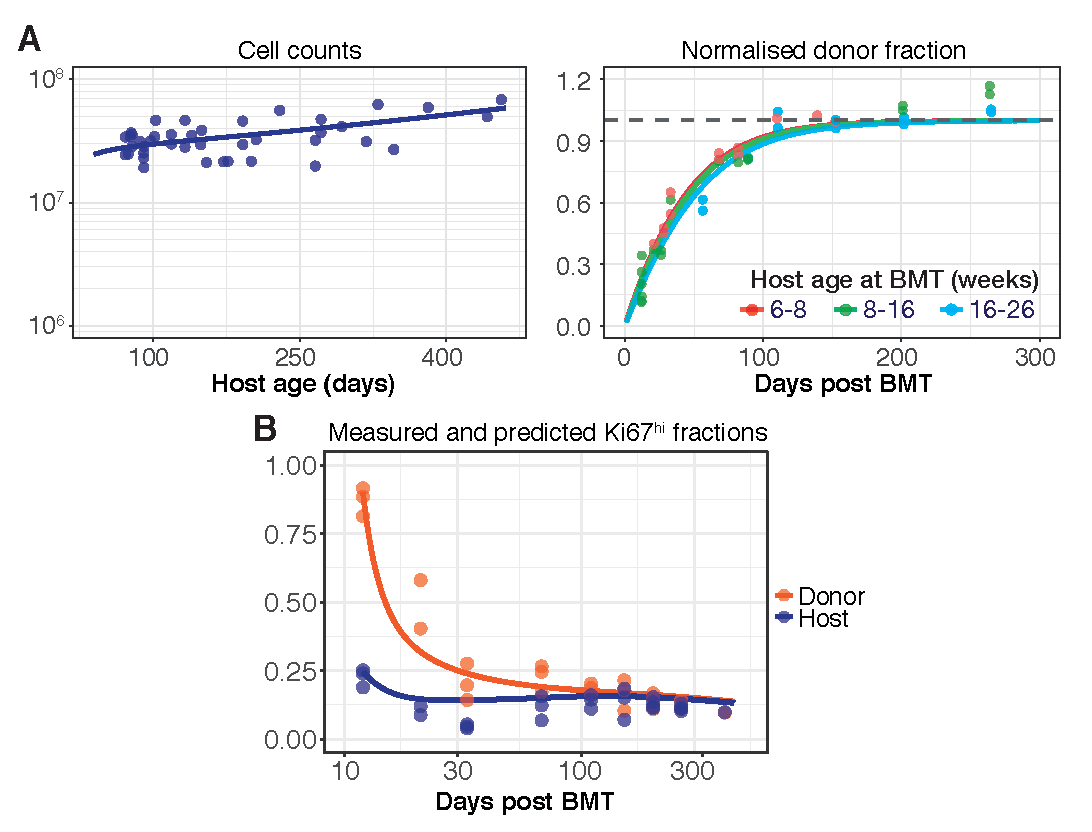
\includegraphics[scale = 0.7] {Results_FM.pdf}}
		\caption{\small \textbf{Fitted and predicted   population dynamics of FM B cells, using the best-fitting model in which cells divide at a constant rate and their mean residence time increases with host age.}  The model was fitted simultaneously to the extended timecourses of total cell counts of FM B cells pooled from LN and spleen in busulfan chimeras, the donor fractions in FM B cells normalised to the chimerism in T1 cells and the proportion of cells that were \khi\ within host and donor FM B cells. Solid lines denote the most probable description of the observations of cell counts and normalised donor fractions and \khi fractions using the time-dependent model with purple envelopes indicating uncertainty in the model fit and the blue envelope indicates uncertainty in the data. Prediction intervals (4.5$^{th}$ and 95.5$^{th}$ percentiles) were plotted by drawing samples from the posterior distribution of parameter estimates.}
		\label{fig:results_FM}
\end{figure}

%\subsection*{The model of time-varying loss successfully predicts the kinetics of Ki67 expression within host and donor populations}
%As well as the numbers of host and donor-derived cells in the FM compartment, we  also measured the kinetics of their expression of Ki67, a nuclear protein expressed during cell cycle and lost with a lifetime of 3-4 days following mitosis (Gossel eLife 2017 \red{and others - see refs in that paper}). Immediately following BMT the donor FM cells are highly enriched for recently divided cells, with around 80\% \khi, but this proportion falls slowly to equalise with that of host cells at around 10\% after approximately 100 days (Figure~\ref{fig:results_FM}C, red and green points).

%As a validation of the models,  which were fitted only to the timecourses of total FM B cell numbers and chimerism, we used them to predict the dynamics of Ki67 expression within host and donor cells over time. The best-fitting time-dependent homogeneous model  predicted these kinetics remarkably well. These predictions were generated by inserting the estimated rates of loss ($\delta(t) = \delta_{0} e^{-rt}$) and division ($\rho$) into a model which explicitly follows the transit of cells between \khi\ and \klo\ states, which we have employed previously (Hogan PNAS 2015, Gossel eLife 2017). We assumed a mean lifetime of Ki67 post-mitosis of 3.5d, and also assumed that \khi\ and \klo\ cells are lost at equal rates $\delta(t)$. The timecourses of host and donor \khi\ fractions were then generated by simulating the model with its best-fit parameters, beginning at the mean \khi\ fractions observed at 12d post-BMT, pooled across all experimental cohorts. See Methods below for details.

%The simulations show that the host/donor disparity in Ki67 expression derives largely from residual expression of Ki67 on cells that have recently entered the FM pool from the T2 precursor population \red{T2s are not dividing, you say... so surely this is further evidence that T1s are the source for FMs?}.  Soon after BMT, the donor FM pool is highly enriched for these recent immigrants, roughly 80\% of which are Ki67,  relative to the more established host-derived pool. The lifetime of FM cells is relatively short and so a substantial fraction of newly immigrated \khi\ cells  are lost before they transition to \klo. This interplay means that quiescent donor cells are slow to accumulate. In parallel, Ki67 levels transiently dip in host FM cells following BMT due to the sudden reduction in influx from the host T2 pool, before they re-establish equilibrium at lower numbers. 

\subsection*{Summary}
\begin{itemize}
	\item Most support for model in which FM B cell residence time increases with host age
	\item No evidence for kinetic heterogeneity (\ie\ multiple subpopulations with different turnover, or host incumbents) 
	%\item No evidence for changes in the per-cell rate of differentiation from T2 with cell age
	\item No evidence for changes in rates of loss or division of FM cells with cell age.
\end{itemize}

%of \khi\ fractions within host and donor compartments .
%The possible explanation for this is that majority of ki67 in FM compartment is source derived suggesting that FM cells are primarily maintained by high influx from source and by very low levels of cell division.
%The high influx corresponds to high loss rate (inverse of residence time, Table~\ref{tab:FM-parestm}) in the FM subset, which only allows for slow accumulation of \klo\ cells post BMT in the donor compartment. 
%Inflow of very high (> 90\% of donor influx) numbers of \khi\ cells with gradual accrual of \klo\ population, temporarily maintains high fractions of \khi\ cells within donor compartment, which slowly stabilise to levels equivalent to that of the host compartment as donor fractions stabilise.
%In the host compartment, since pre-existing cells are mostly \klo, the low inflow ($\chi \sim$ 0.8)  of new \khi\ cells doesnt alter the kinetics of \khi\ fractions within these cells.
%In summary, we find no strong evidence for heterogeneity within FM B cells which are suggested to be firmly regulated by the homeostatic factors changing with the age of the host.
	
%: Table 1
	\begin{table}[h!]
		\begin{center}
			\renewcommand{\arraystretch}{1.25}
			\begin{tabular}{c c c c c} 
				\toprule 
				\multicolumn{4}{c}{\textbf{Model and $\Delta$Loo-ic}} \\
				\cline{2-5}
				 Source &{\small Time-dependent}  & {\small Simple homogeneous} &  {\small Kinetic heterogeneity} & {\small Incumbent} \\ 
				\toprule
				    T1    &   0             &              8             &                7              &          9         \\ 
				    T2    &   36            &              43            &                39             &          42        \\ 
			      T1 + T2 &   19            &              29            &                28             &          29        \\ 
				\hline
				\toprule 
			\end{tabular}
		\end{center}
		\caption{\small \textbf{Comparison of models describing population dynamics of Follicular Mature (FM) B cells, pooled from LN and spleen}. Loo-ic values obtained using leave-one-out cross validation method are shown relative to that of the best fitting model, in which the rate of loss  (turnover) of FM cells declines slowly with the age of the host. Predictions of more complex models were very close to those of the simple homogenous model (that is, either very little kinetic heterogeneity, close to zero incumbent cells, or effects of cells age on turnover or division rates)}. 
		\label{tab:FM-AICs}
	\end{table} 
	
	\vspace{1cm}
	
	
%: Table 2
	\begin{table}[h!]
		\begin{center}
			\renewcommand{\arraystretch}{1.25}
			\begin{tabular}{ l r l } 
				\toprule 
				\textbf{Parameter}  &  {\small Estimate}  &  {\small 95\%  $^{\ast}$CI} \\ 
				\toprule
				Total cell numbers at age 7 wks ($\times 10^{-6}$)      & 32       &  (24, 43)  \\ 
				Percent daily replacement by source at age 8.5 wks      & 2.7      &  (2.3, 3.0)  \\
				Mean residence time (days) at age 7 wks                 & 31       &  (24, 39)  \\ 
				Mean inter-division time (days)                         & 291      &  (129, 2200)  \\
				Time for mean residence time to double (days)           & 204      &  (118, 622)  \\
				Average time of loss of Ki67 expression (days)          & 6.0      &  (4.6, 7.3)  \\
				\hline
				\toprule 
			\end{tabular}
		\end{center}
		\caption{\small \textbf{Parameter estimates from the best-fit (time-dependent) model for FM B cells (Spleen + LN)}. $^{\ast}$Credible intervals were estimated by taking 2.5$^{th}$ and 97.5$^{th}$ percentiles of the posterior probability distribution of the parameter values obtained after fitting model to the data.}
		\label{tab:FM-parestm}
	\end{table} 
	
\clearpage
	
\section*{Germinal Center B cells}

\subsection*{Invasion kinetics of donor-derived GC cells differ between spleen and lymph nodes.}
GC cells are known to derive directly from the mature follicular cells [REF] which circulate freely between spleen and lymph nodes [ref].
Therefore, we used pooled numbers of spleen and LN FM cells as a common source for all GC B cell subsets.
We found that in both spleen and lymph nodes, the chimerism in GC compartment reaches to the level of chimerism in their source (FM) population (Figure \ref{fig:results_GC} B), showing complete replacement of host GC cells by that of donor-derived cells. 
%This suggests that the host and donor GC cells follow the same rules of turnover.
Surprisingly, the chimerism in splenic GC cells stabilises twice as fast than their lymph node counterparts ($\sim$120 days for spleen GCs versus $\sim$250 days for LN GCs). 
Due to this  disparity in the invasion kinetics of donor cells between the splenic and LN GC pools, we model them separately assuming that circulating FM cells feed into both these populations with a constant rate over time. 

\subsection*{B cells participating in GC reactions follow same kinetics of division and loss, irrespective of the age of the host.}
To understand the behaviour of GC B cells we began with the simplest model, where all cells are assumed to divide and turnover with constant rates at all times, thereby implying homogeneity.
This simple homogeneous model provided good visual descriptions of time-courses of cell counts and normalised donor fraction (Figure~\ref{fig:results_GC}) with estimates of mean resident times of 0.6(0.48, 0.8) and 0.8(0.59, 1.1) days for spleen and LN GCs respectively.
The simple model with constant rates of cell-division and turnover also captured the trend in \khi fractions in host and donor compartments of splenic and LN GC populations remarkably well ( Figure~\ref{fig:results_GC} ). 
We also found that GC cells enter divisions very frequently with average times between cell cycles $\sim$0.6 and $\sim$0.8 days for spleen and LN GC cells, respectively.
Majority of the GC precursors (FMs) have fewer \khi cells ($\simeq$ 10\%), we speculate that almost all of the GC cells undergo multiple rounds of cell-division or are lost from the pool rapidly before losing their Ki67 expression or both.

%This shows that individual B cell clones persist  $\sim$3 times longer in lymph node germinal centres, while in spleen they are lost relatively rapidly (mean clonal lifetime = 42 and 13 days for spleen and LN GCs respectively, Table~\ref{tab:GC-parestm}). 
We observed that $\sim$0.3\% of LN GC and $\sim$57\% of spleen GC population is replaced everyday by new cells seeding in from the follicular compartment.
The estimate of substantially higher source influx into spleen GC pool is consistent with the observation of quicker stabilisation of chimerism in spleen GC cells as compared to LN GC cells. 
It can be inferred from this analysis that GC reactions have disparate half-lives between different secondary lymphoid organs and their dynamics are primarily regulated by tissue-specific factors.

We further tested weather varying either division or turnover with time improves on the fits provided by the simple homogeneous model. 
Allowing variations in $\rho$ or $\delta$ with host age did not enhance the quality of fits and received poorer statistical support ($\Delta$LOO-IC$_{\rho}$ = ? and 5 and$\Delta$LOO-IC$_{\delta}$ = 0 and 4.9  for splenic and LN GCs, respectively) as compared to the simple homogeneous model. 
Additionally, the rates of change of $\rho$ or $\delta$ estimated by the time-dependent model were extremely small with confidence intervals spanning across zero, suggesting that the given data can be explained without any changes in division or turnover. % showing large uncertainty in parameter estimates.
Therefore, we speculate that the time-dependent variations in the host environment have little or no effect on the population dynamics of B cells participating in GC reactions.
% $\lambda$ gives the ability of individual clones to persist in the GC follicles.


\subsection*{GC population is maintained by continuous seeding of follicular cells into a kinetically homogeneous population over time.}
The complete replacement that we see in GC cells can also be explained by the presence of kinetically heterogeneous subpopulations that divide and turnover at different but constant rates. 
This model of kinetic heterogeneity assumes that the GC population is comprised of fast and slow subsets (as discussed in FM B cells section).
%The differences in dynamics of these subpopulations result in initial rapid increase in donor fractions followed by slower kinetics that lead to stabilisation to the same levels of donor fractions as seen in the source compartment. 
We found that the kinetic heterogeneity model failed to improve on the fits from simple homogeneous model ($\Delta$LOO-ic = 0 and 1.1 for spleen and LN GCs respectively, Table~\ref{tab:GC-AICs}) and produced  strikingly similar estimates of loss rates and division rates for both fast and slow subsets in both spleen and LN GC cells.

We also tested the variant of the kinetic heterogeneity model where the host and donor cells behave differently due to the presence of a persistent incumbent subpopulation in the host compartment.
We assume that this incumbent population is established during neonatal stages as the early waves of self-renewing B cells populate the peripheral compartments that are resistant to displacement by new cells.
The incumbent model returned visually similar fits to the time-course of total counts and normalised donor fractions as that of the simple homogeneous model (not shown).
It also failed to differentiate from the simplest model statistically despite having an extra parameter (Table~\ref{tab:GC-AICs}).
Moreover, the estimates of loss and division rates ($\delta_{\text{INC}}$ and $\rho_{\text{INC}}$) of the incumbent population were nearly equal to the loss and division rates of the displceable subset, showing very weak signature of heterogeneity.
These results favour the possibility that GC populations despite being extremely dynamic are kinetically homogeneous and are sustained by constant feeding from follicular B cells.

%Each instance of GC reaction typically lasts for about 3-4 weeks [Can kesmir and Rob de Boer JI 1999, L. Mesin et al., Immunity 2016].
%During this period individual GC B cells undergo massive expansions and intermittent selection events followed by the rapid collapse of GC clusters. %[Nilushi De Silva and Ulf Klein, Nat. Rev. Imm. 2015, N. Wittenbrink  et al., JI 2010]. 
%This suggests that the majority of GC B cells are short-lived and it is less likely that their turnover or division rates are influenced by the cell-intrinsic changes accumulated over their short stay in germinal centres.
%Therefore, we refrained from using more complex models that allow either the cell-division or turnover of GC B cells to vary with cell-age.
%\red{I have fitted the age-structured model on GC cells and it fails to fit to LN GCs and show $\Delta$ AIC of 380 in spleen GCs.}

Our analysis of FM population dynamics shows that the total size of FM compartment increases with time, due to a gradual decline in their turnover (Figure \ref{fig:results_FM}A, left panel).
We tested whether the rate of influx of FM cells into the GC compartment also varies with host-age, so as to maintain the inflow of constant number of cells over time. 
%The time-dependent changes in the influx rate of FM cells in kinetically homogeneous GC compartment may explain the gradual slow down of donor cell invasion in the GC pool.
We found that allowing the rate of influx to vary with host-age, results in very poor descriptions of the normalised donor fractions in both, spleen and LN GC populations ($\Delta$ LOO-ic of ?? and ?? respectively) and hence rejected this possibility.
\red{Therefore, follicular cells maturing into the GC compartment at any given time are proportional to the size of the FM population at that moment.}


%\subsection*{GC B cells maintain high Ki67 expression by active division and rapid turnover.}
%As described earlier for FM cells, we used an additional validation strategy to test the robustness of the model with the best-fit to cell counts and normalised donor fractions, by comparing its predictions of \khi fractions to the observed data.
%GC populations in both, spleen and lymph nodes, are always highly enriched for recently divided cells with more than 90\% cells expressing high levels of Ki67 throughout the timecourse that we studied.
%We analysed the transition of GC cells between \khi and \klo subsets by solving the equations described in~\ref{eq:ode_ki67}, separately for the host and donor compartments. 
%The rate of influx of FM cells into the GC compartment changes very slowly (it takes $\sim$ a year for the number of FM cells maturing into GC compartment to fall by a factor of two), which allows us to assume that the \khi and \klo GC subsets are in the state of quasi-equilibrium.
%We could then simulate the model described in eq.~\ref{eq:ode_ki67} using the rates of cell-division and turnover of \khi and \klo subsets inferred from the estimates of mean clonal lifetimes (Table~\ref{tab:GC-parestm}) of splenic and LN GC cells (detailed description in methods and Hogan et al. PNAS 2015).

%
%These predictions were made by assuming that the recently divided cells lose their post-mitotic Ki67 expression by $\sim$ 3.5 days [Gossel et al., eLife 2017] and also that the cell-division event does not alter the ability of cells to persist in GC compartments. 
%Since, 


\subsection*{Summary/Discussion}
\begin{itemize}
	\item GC cell dynamics vary between spleen and lymph nodes, as observed by slower replacement kinetics of LN GC cells  as compared to their splenic counterparts.
	Accordingly, our analysis predicts longer persistence of GC cells in lymph nodes than in spleen.
	
	\item Simple homogeneous model with constant rates of cell-division and turnover explains GC cell dynamics and predicts the kinetics of \khi fractions remarkably well, in both spleen and lymph nodes.
	This may suggests that under the influence of very strong antigen derived signals the mean inter-division and residence times of all cells within the GC pool, remain constant across different instances of germinal centre reactions, over time.
	The strong signals from antigen and T helper cells wash out the time-variability in turnover of their precursors (FMs)?
	
	\item Prolong GC reactions in response to viral antigens and gut microbes (Adachi et al. 2015, Bachman et al. 1996, Kasturi et al. 2011) may allow B cells to reach higher degree of affinity maturation $\rightarrow$ means to cope with constant antigenic drifts. 
	An important question is whether chronic GC response consists of long-lived GC cells or constant invasion of short lived cells maintaining a long-lived steady state? Our analysis favours second scenario. 
	
	\item Ki67 in GC is result of active division and turnover and is not source derived. FM population has 10\% \khi cells while GC are $\sim$ 95\% \khi. 
\end{itemize}



\begin{figure}[h!]
	\centerline{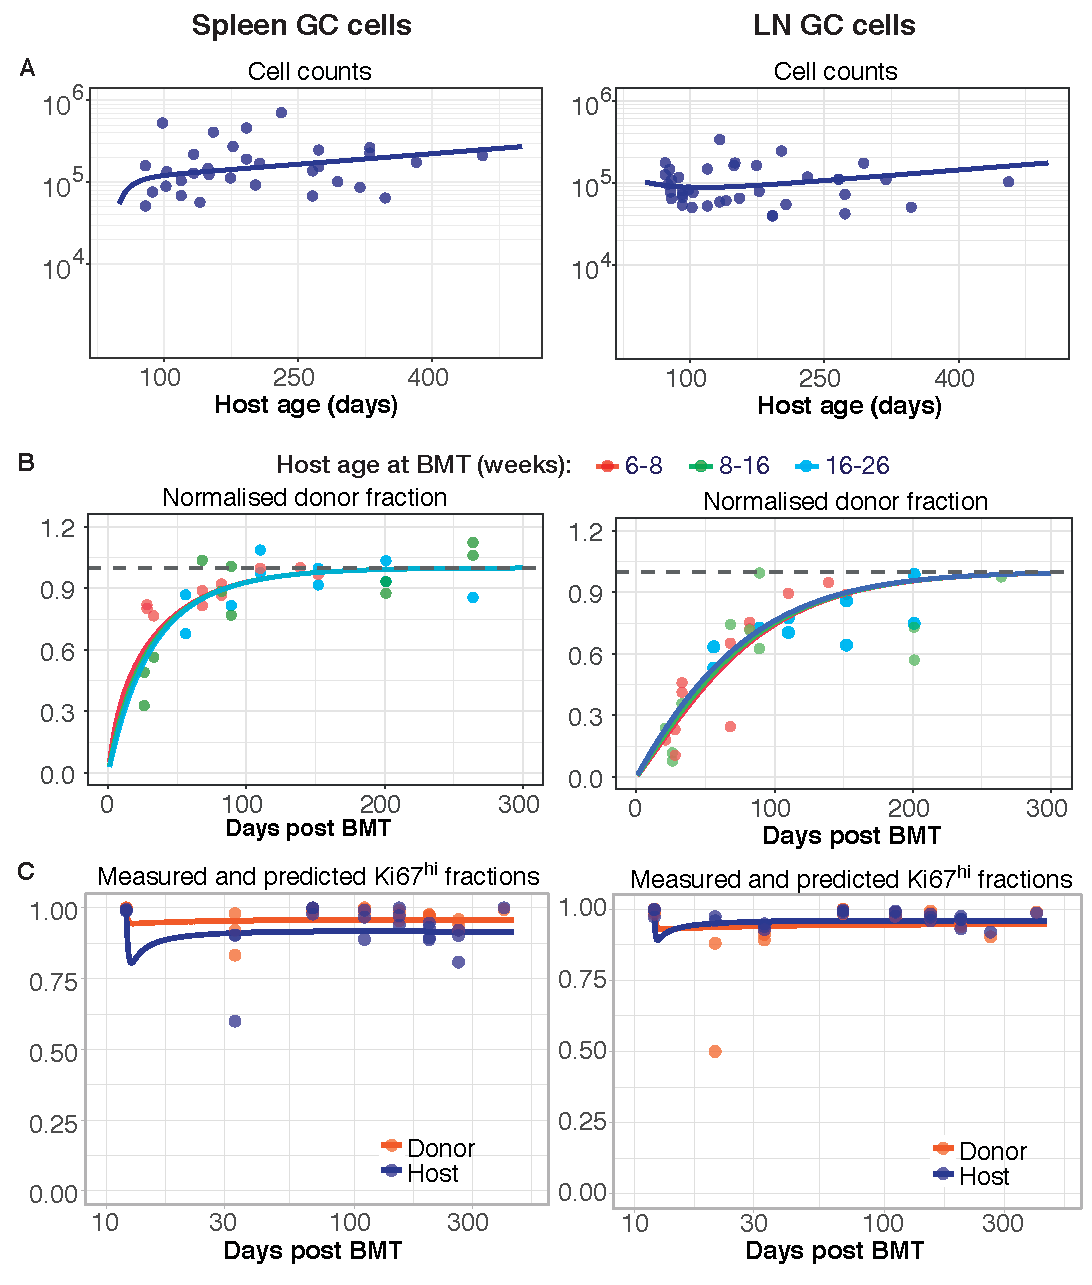
\includegraphics[scale = 0.8] {Results_GC.pdf}}
	\caption{\small \textbf{Fitted and predicted population dynamics of spleen and LN GC B cells, using the best-fitting model in which cells the net loss rate of cells remain constant with time.}  The model was fitted simultaneously to the extended time-courses of total cell counts of spleen and LN GC B cells pooled in busulfan chimeras, the donor fractions normalised to the chimerism in FM B cells and the proportions of \khi cells within their host and donor compartments. Solid lines are the fit from the simple-homogeneous model to the observations (closed circles) of cell counts, normalised donor fractions and the proportion of cells that were \khi\ within host and donor spleen and LN GC B cells, with orange envelopes indicating uncertainty in the model while blue envelope indicate uncertainty in the data. Prediction intervals (4.5$^{th}$ and 95.5$^{th}$ percentiles) were plotted by drawing samples from the posterior distribution of parameter estimates.}
	\label{fig:results_GC}
\end{figure}

%: Table 1
\begin{table}[h!]
	\begin{center}
		\renewcommand{\arraystretch}{1.25}
		\begin{tabular}{ l c c c c} 
			\toprule 
			& \multicolumn{4}{c}{\textbf{Model and $\Delta$Loo-ic}} \\
			\cline{2-5}
			\textbf{population}  &  {\small Simple homogeneous}   & {\small Time-dependent} &  {\small Kinetic heterogeneity} & {\small Incumbent}   \\ 
			\toprule
			LN GC cells         & 0   &  4.9  & 1.1 & 2.9   \\ 
			Spleen GC cells     & 0   &  0    & 0   & 1  \\ 			
			\hline
			\toprule 
		\end{tabular}
	\end{center}
	\caption{\small \textbf{Comparison of Loo-ic values obtained using leave-one-out cross validation method are shown for different models fitted to cell counts and donor fractions in spleen and LN GC B cells normalised to the chimerism in FM cells (spleen + LN).}} 
\label{tab:GC-AICs}
\end{table} 

%: Table 2
\begin{table}[h!]
	\begin{center}
		\renewcommand{\arraystretch}{1.25}
		\begin{tabular}{l l r l } 
			\toprule 
			\textbf{Population} & \textbf{Parameter}  &  {\small Estimate}  &  {\small 95\% CI$^{\ast}$} \\ 
			\toprule
			\textbf{Lymph node GC cells} & Total cell numbers at age 8.5 wks ($\times 10^{-3}$)     & 62      &  (23, 188)    \\ 
			& Percent daily replacement by source at age 8.5 wks                                    & 3.3     &  (2.8, 3.5)   \\
			& Mean resident time (days)                                                             & 0.80    &  (0.58, 1.1)  \\ 
			& Mean inter-division time (days)                                                       & 0.80    &  (0.59, 1.1)  \\ 	
			& Average time of loss of Ki67 expression (days)                                        & 5.6     &  (4.2, 7.2)  \\		
			\textbf{Splenic GC cells} & Total cell numbers at age 8.5 wks ($\times 10^{-3}$)        & 7.2     &  (1.8, 30)    \\ 
			& Percent daily replacement by source at age 8.5 wks                                    & 57      &  (38, 97)   \\
			& Mean resident time (days)                                                             & 0.61    &  (0.49, 0.80)  \\ 
			& Mean inter-division time (days)                                                       & 0.60    &  (0.48, 0.79)  \\ 	
			& Average time of loss of Ki67 expression (days)                                        & 6.2     &  (4.9, 7.7)  \\		
			\hline
			\toprule 
		\end{tabular}
	\end{center}
	\caption{\small \textbf{Parameter estimates from the best-fit (simple homogeneous) model for spleen and LN GC B cells.}  $^{\ast}$Credible intervals were estimated by taking 2.5$^{th}$ and 97.5$^{th}$ percentiles of the posterior probability distribution of the parameter values obtained after fitting model to the data.}
	\label{tab:GC-parestm}
\end{table} \



\end{document}




